\chapter{Predictive Reconfiguration Control for Multi-Robot Formation in Cluttered Environments}\label{paper3}

\noindent{\normalsize Submitted in:\\
\textit{IEEE Transactions on Control of Network Systems}\\
Code: {\tt\url{https://github.com/duynamrcv/prc}}\\
Video: {\tt\url{https://youtu.be/oAhgOOhFSCA}}
}
\vspace{1cm}

% \noindent\textit{\textbf{Abstract}}

% Reconfiguration control is essential for multi-robot systems to adapt their formations in response to environmental conditions when carrying out complex tasks. This chapter introduces a novel approach called predictive reconfiguration control (PRC) to navigate a swarm of robots through cluttered environments with narrow passages such as valleys or tunnels. The robot swarm is modeled as a directed sensing graph where each node represents a robot capable of collecting real-time data on the environment and the states of nearby robots within its communication range. The information from each node is used as input to the controller to adjust its parameters in two control modes, \textit{``formation''} and \textit{``tailgating''}, which serve as the basis for formation adaptation. A set of cost functions is then introduced to represent swarm constraints, including formation shape, reference speed, movement direction, and collision avoidance. These cost functions also allow for the prediction of the swarm's states so that model predictive control solvers can be used to minimize the cost for optimal control signals. Results from a number of comparisons and evaluations show that the proposed controller is not only capable of navigating the robot swarm through challenging environments with narrow passages but also outperforms other state-of-the-art formation control techniques in most performance metrics. Software-in-the-loop tests have been conducted to verify the validity of the proposed controller for practical scenarios.
% % \end{abstract}

% \noindent\textbf{\textit{Keywords:}}
% formation control, multi-robot system, distributed control, reconfiguration control, model predictive control
% \end{keywords}

This chapter presents an optimal solution of the ERC, which is presented in Chapter~\ref{paper2} called predictive reconfiguration control (PRC) to navigate a swarm of robots through cluttered environments with narrow passages such as valleys or tunnels. A set of cost functions is introduced to represent swarm constraints, including formation shape, reference speed, movement direction, and collision avoidance. These cost functions also allow for predicting the swarm's states so that model predictive control solvers can be used to minimize the cost for optimal control signals.

\section{Introduction}
Formation control of multiple robots is becoming increasingly important due to its capability to perform challenging tasks in complex environments such as disaster response, search and rescue, tracking of multiple targets, and swarm-based reconnaissance~\cite{9306908,Oh2015}. This approach also enhances system resilience as any malfunction within the swarm can be mitigated by reconfiguring the formation. The reconfiguration also enables the swarm to navigate through cluttered environments where a fixed topology is insufficient to adapt the formation to varying conditions. Formation reconfiguration control therefore is essential to ensure the effective operation of a robot swarm.

In formation control, a popular approach is based on natural collectives, such as school of fish or flocking of birds~\cite {Nagy2010}, where movement is driven by a set of simple behaviors: \textit{repulsion} that steers an agent away from its neighbors; \textit{cohesion} that attracts the agent to the group; \textit{migration} that orients its motion in a preferred direction; and \textit{obstacle repulsion} to avoid collisions~\cite{Reynolds1987}. Those behaviors are often used with artificial potential fields (APF) to produce control signals for each robot~\cite{736776,Berlinger2021,9565893, 7434587}. In particular, formation and navigational behaviors are combined in~\cite{736776} as concurrent asynchronous processes to guide a group of robots to reach their goals in a desired formation. In~\cite{Berlinger2021}, the AFP is used to coordinate behaviors among fish-inspired miniature underwater robots to obtain  
collective capabilities without having direct communication. However, behavior-based methods are limited in guiding the swarm through complex environments because a set of fixed behaviors lack the flexibility to handle abrupt changes in the environment~\cite{Zhang2023}.

To address this limitation, several studies propose a hybrid approach that combines the AFP with optimization techniques to better integrate behaviors. For example, the APF is used with an artificial neural network in~\cite{Elkilany2020} to optimize potential force parameters so that the swarm can adapt to environmental conditions. Similarly, an evolutionary optimization framework is introduced in \cite{Vsrhelyi2018} to select parameters and fitness functions that enhance the velocity and cohesion of the swarm. Nevertheless, optimizing parameters is insufficient to address the main problem of the behavior-based approach, which depends on a set of fixed behaviors. 

Recently, an approach using optimal control to manage swarm constraints and predict agents' states has been introduced for reliable formation~\cite{Beaver2021,Soria2021,8950150}. In~\cite{7828016,Wu2020}, optimization-based motion planners are used for individual point-to-point transitions to maintain the formation shape while avoiding collisions in multi-robot systems. In~\cite{Soria2021}, model predictive control (MPC) is introduced for swarm navigation in which cost functions and constraints are used to regulate speed, ensure safety, and guide the drones through the environment. The system however is centralized and dependent on a primary agent. A distributed MPC in~\cite{9562281} offers decentralized computation for formation control, but it is only practical in spacious cluttered environments. Maintaining a specific formation shape in tight spaces is challenging due to conflicts between shape preservation and collision avoidance. 

In another direction, several studies propose control techniques that reconfigure the formation in response to sudden changes in the environment structure \cite{AlonsoMora2018,9013071,9981858,10417519}. In~\cite{AlonsoMora2018}, a distributed method capable of reconfiguring the formation is introduced for environments with both static and dynamic obstacles. The method computes a movable convex region from the robots' current positions and then repositions them within this region based on the desired movement direction. However, the transition relies on reassigning robots to predefined virtual points on the reference formation rather than utilizing information obtained from the environment. In~\cite{9981858}, affine transformations are used to modify formation shapes for obstacle avoidance in dense environments, but they require information to be shared among all the robots. Our previous work~\cite{10417519} adapts a V-shape formation to guide a robot swarm through narrow corridors. The two wings of the V-shape can expand or contract to form a suitable shape based on real-time information about the available space. Nonetheless, this approach has not considered the physical limits of the robots, which could lead to infeasible control inputs and unexpected collisions in certain scenarios. Besides, the ability of each robot to make decisions based on local sensor data remains limited.

Building upon recent progress in multi-robot formation, this work introduces a novel technique named predictive reconfiguration control (PRC) for safe and effective navigation of a decentralized multi-robot swarm in cluttered environments. The robots are equipped with local sensors and communication modules to collect information about the environment and the states of their neighboring robots. The PRC is implemented on each robot to enable adaptive formation capabilities. The contributions of this work are threefold:
\begin{enumerate}
    \item Model the formation as a directed sensing graph where each node represents a robot capable of sensing its surroundings and communicating with its neighbors. This representation allows the system to be decentralized and the formation to be formulated as an optimization problem.
    \item Define a set of cost functions that represent the formation constraints and performance. The functions ensure not only the desired formation shape but also the swarm's performance, including the desired velocity, direction, and obstacle avoidance. The cost functions are designed to be compatible with existing solvers for MPC, thereby simplifying the implementation.
    \item Propose a predictive reconfiguration controller with two modes, \textit{``formation''} and \textit{``tailgating''}, capable of adapting the formation shape in response to environmental changes. Extensive simulations and comparisons have been conducted to evaluate the robustness, scalability, and effectiveness of the proposed controller. Software-in-the-loop tests have also been conducted to verify its practical applicability. The source code of the proposed controller is publicly available for further research and practical implementation.
\end{enumerate}

The remaining sections of this chapter are organized as follows. Section~\ref{sec:problem} describes the formation model. Section~\ref{sec:propose} presents the proposed formation reconfiguration control method. Section~\ref{sec:result} shows simulations, comparisons, and software-in-the-loop experimental results. The paper ends with conclusions drawn in Section~\ref{sec:conclusion}.

\section{Formation Background}\label{sec:problem}
Consider a swarm $\mathcal{N}$ of $N$ robots labeled $i\in\left\{1,...,N\right\}$. The swarm is modeled as a directed sensing graph $\mathcal{G}=\left(\mathcal{V},\mathcal{E}\right)$, where vertex set $\mathcal{V} = \left\{1,..., N\right\}$ represents the robots, and edge set $\mathcal{E}\subseteq\mathcal{V}\times \mathcal{V}$ includes robot pairs $\left(i, j\right)\in\mathcal{E}$ for which robot $i$ can sense robot $j$. Denote $\mathcal{N}_i=\left\{j\in\mathcal{V}|\left(i,j\right)\in\mathcal{E}\right\}\subset\mathcal{V}$ as the set of $N_i$ neighbors of a robot $i$ in $\mathcal{G}$.

In this work, the dynamics of the robots are represented in discrete time. Denote $p_i(k),v_i(k),u_i(k)\in\mathbb{R}^3$ respectively be the position, velocity and control input of robot $i$ at time $t(k) = k\tau$, where $\tau$ is the sampling period. The robots in the swarm are homogeneous with a body radius $r$. Each robot is equipped with an inertial measurement unit (IMU) to determine its position and orientation, a range sensor to scan the environment, and a wireless ad-hoc network module to carry out peer-to-peer communication with other robots. In this work, the communication delay between each pair of robots is negligible~\cite{AlonsoMora2018,9527169}. The range sensor provides a $360^\circ$ field of view with the scanning area $S_s$ of radius $r_s$, as shown in Figure~\ref{fig:model}. Its point data obtained at time $t(k)$ is represented by set $\mathcal{M}_i(k)=\left\{m\right\}$.
\begin{figure}
    \centering
    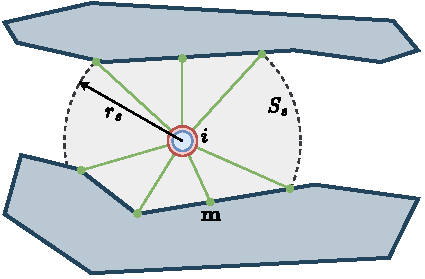
\includegraphics[width=0.48\textwidth]{paper3/images/model.pdf}
    \caption{Illustration of a robot with its range sensor having the scanning area $S_s$ (dashed gray circle) of radius $r_s$ and set $\mathcal{M}_i=\{m\}$ (green) of the acquired point data.}
    \label{fig:model}
\end{figure}

According to~\cite{Soria2021}, the robot in the swarm can be represented as a discrete linear system as follows:
\begin{equation}
    x_i(k+1)=A_ix_i(k) + B_iu_i(k),
\end{equation}
where $A_i$ and $B_i$ are system matrices, $u_i$ is input acceleration, and $x_i=\left[p_i;v_i\right]\in\mathbb{R}^6$ is a state vector including position and velocity. The velocities and accelerations are bounded, i.e., $v_\text{min}\leq v_i(k)\leq v_\text{max}$ and $u_\text{min}\leq u_i(k)\leq u_\text{max}$.
\section{Predictive Reconfiguration Control}\label{sec:propose}

\begin{figure}
    \centering
    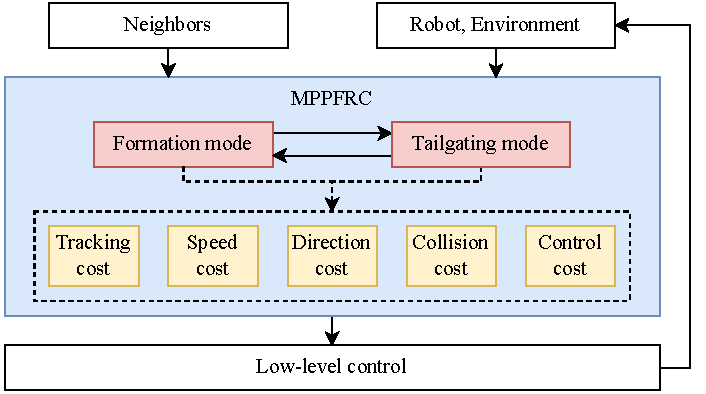
\includegraphics[width=0.7\textwidth]{paper3/images/diagram.pdf}
    \caption{Diagram of the proposed predictive reconfiguration control strategy.}
    \label{fig:diagram}
\end{figure}

The aim of reconfiguration control is to drive the robot swarm through a cluttered environment having narrow passages. The swarm adheres to the following constraints: (\textit{C1}) maintain certain desired shapes; (\textit{C2}) move along a prioritized direction $\mathbf{u}_\text{ref}\in\mathbb{R}^{3}$; (\textit{C3}) obtain the desired speed $\bar{v}_\text{ref}\in\mathbb{R}$; and (\textit{C4}) ensure no collision with other neighbors or obstacles in the environment. To address this problem, we propose a predictive reconfiguration control system as shown in Figure~\ref{fig:diagram}. Inputs to this system include point cloud data from range sensors and the states of neighbor robots. Depending on the environment structure inferred from the point cloud data, the controller operates in either the \textit{``formation''} or \textit{``tailgating''} mode. The \textit{``formation''} mode maintains the desired shape, whereas the \textit{``tailgating''} mode transforms the formation into a line to navigate through narrow spaces like valleys or tunnels. The controller is designed based on a weighted-sum of five cost functions to meet constraints $(C1)-(C4)$. An optimal solver is then used to generate control signals for low-level controllers.

Let $\delta_{ij}\in\mathbb{R}^3,\forall j\in \mathcal{N}_i$ be the vector representing the desired position of robot $i$ with respect to neighbor $j$. The formation is obtained via the following constraint~\cite{Dong2016,6798711}:
\begin{equation}
    \lim_{k\to\infty}{\left(\mathbf{p}_j(k)-\mathbf{p}_i(k)+\kappa\delta_{ij}\right)}=0,\quad\forall i,j\in\{1,...,n\}, i\neq j
\end{equation}
where $\kappa\in[0,1]$ is a scaling factor representing the shrinkage level of the formation. The desired relative position of robot $i$ in the formation is then described as:
\begin{equation}
    \mathbf{p}^*_i(k)=\dfrac{1}{n_i}\sum_{j\in\mathcal{N}_i}{\left(\mathbf{p}_j\left(k\right)+\kappa\delta_{ij}\right)}.
    \label{eqn:formation}
\end{equation}

During the transition between modes, each robot determines a leader as a reference to determine its position. The leader is selected based on the inner product $\tilde{\mathbf{p}}_{ij}$ of the difference between robot $j$ in the neighbor set $\mathcal{N}_i$ and robot $i$, $\mathbf{p}_j-\mathbf{p}_i$, and the desired direction, $\mathbf{u}_\text{ref}$, as follows:
\begin{equation}
    \tilde{\mathbf{p}}_{ij} = \left\langle (\mathbf{p}_j-\mathbf{p}_i),\mathbf{u}_\text{ref}\right\rangle.
    \label{eqn:tildep}
\end{equation}

A positive value of $\tilde{\mathbf{p}}_{ij}$ indicates that robot $j$ is in front of robot $i$ in the $\mathbf{u}_\text{ref}$ direction, and vice versa. Let $\mathcal{P}_i$ be the set of inner products for all robots $j$ in the neighbor set $\mathcal{N}_i$, $\mathcal{P}_i=\left\{\tilde{\mathbf{p}}_{ij}\right\}$. Leader robot ${l_i}$ of robot $i$ is chosen as the closest robot in front of it, i.e.,
\begin{equation}
     l_i=\begin{cases}
    \arg\min_{j}\left\{\tilde{\mathbf{p}}_{ij}\in\mathcal{P}_i\vert\tilde{\mathbf{p}}_{ij}\geq0\right\} & \exists~\tilde{\mathbf{p}}_{ij}\geq0\\ 
    -1 & \text{otherwise}
     \end{cases}
    \label{eqn:li}
\end{equation}

\begin{algorithm}
\caption{Pseudocode of the leader selection}
\label{alg:ls}
\ForEach{$j\in\mathcal{N}_i$}{
    Compute inner product $\tilde{\mathbf{p}}_{ij}$\tcc*[r]{Eq. \ref{eqn:tildep}}
    $\mathcal{P}_i\leftarrow\tilde{p}_{ij}$\;
}
Select leader $l_i$ for robot $i$ to follow\tcc*[r]{Eq. \ref{eqn:li}}
\Return $l_i$\;
\end{algorithm}

Algorithm~\ref{alg:ls} presents the leader selection process. 

In the \textit{``tailgating''} mode, robot~$i$ needs to align and keep a distance~$d_\text{ref}\in\mathbb{R}$ with its leader~$l_i$. This can be formulated as follows:
\begin{equation}
    \lim_{k\to\infty}{\left\Vert \mathbf{p}_{l_i}(k)-\mathbf{p}_i(k)\right\Vert}=d_\text{ref}
    \label{eqn:tailcon}
\end{equation}
The desired relative position of robot~$i$ then can be determined as follows:
\begin{equation}
    \mathbf{p}_i^*(k)= \mathbf{p}_{l_i}(k)-d_\text{ref}\mathbf{u}_\text{ref}.
    \label{eqn:tailgating}
\end{equation}

Using equations \eqref{eqn:tildep} and \eqref{eqn:tailgating}, the formation problem is converted into tracking the desired position $\mathbf{p}_i^*$, which can be handled by predictive controllers. 

\subsection{Predictive control design} 
\begin{figure*}
    \centering
    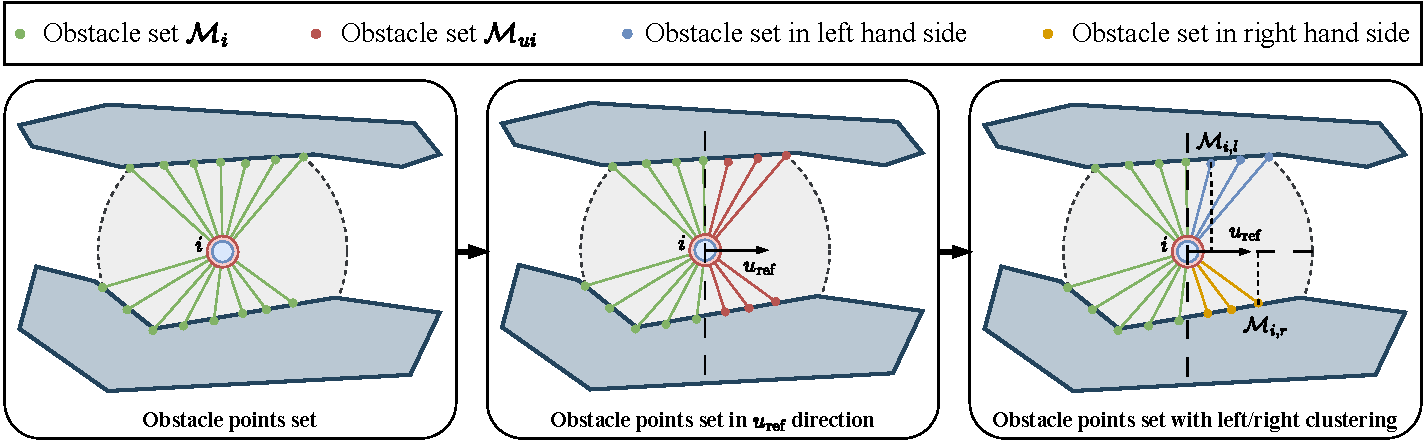
\includegraphics[width=\textwidth]{paper3/images/perception.pdf}
    \caption{The process of estimating the environment's width from the robot's range sensor.}
    \label{fig:perception}
\end{figure*}
The proposed predictive controller uses the desired position $\mathbf{p}_i^*$ as the reference and a set of cost functions to fulfill formation constraints $(C1)-(C4)$. The functions include tracking cost $J_{t,i}$, direction cost $J_{d,i}$, speed cost $J_{s,i}$, obstacle avoidance cost $J_{o,i}$, inter-agent collision cost $J_{i,i}$, and control effort cost $J_{u,i}$. Let $P\in\mathbb{N}^+$ be the prediction horizon, which is finite and shifts forward at each time step; $(\cdot)(k+l|k )$, $l \in\{0,...,P\}$, be the predicted value of $(\cdot)(k+l )$ when the information at time $t(k)$ is available; $\mathbf{X}_i(k)\in\mathbb{R}^{6P}$ be the sequence of the predicted states $\mathbf{x}_i(k+l|k)$ over the horizon $l\in\{1,...,P\}$; and $\mathbf{U}_i(k)\in\mathbb{R}^{3P}$ be the sequence of the predicted control inputs $\mathbf{u}_i(k)$ over the horizon $l\in\{0,...,P-1\}$. The predictive reconfiguration control can be modeled as a non-convex optimization problem as follows:
\begin{equation}
    \min_{\mathbf{U}_i(k)}\left(J_{t,i}(k)+J_{s,i}(k)+J_{d,i}(k)+J_{o,i}(k)+J_{i,i}(k)+J_{u,i}(k)\right)
    \label{eqn:J}
\end{equation}
subject to:
\begin{equation}
    \begin{aligned}
        &\mathbf{x}_i(k+l+1|k)=\mathbf{A}\mathbf{x}_i(k+l|k)+\mathbf{B}\mathbf{u}_i(k+l|k),\\
        &\mathbf{x}_i(k|k)=\mathbf{x}_i(k),\\
        &\mathbf{v}_\text{min}\leq \mathbf{v}_i(k+l|k)\leq \mathbf{v}_\text{max},\\
        &\mathbf{u}_\text{min}\leq \mathbf{u}_i(k+l|k)\leq \mathbf{u}_\text{max},\\
    \end{aligned}
    \label{eqn:constraints}
\end{equation}
with $l\in\{1,...,P\}$, and $i\in\mathcal{N}$. The cost functions are defined as follows.

\subsubsection{Tracking cost}\label{sec:tracking_term}
The tracking term aims to drive the robots toward their reference positions to achieve the desired formation shape. It is defined as the square error between the desired position~$\mathbf{p}_i^*$ and the predicted position~$\mathbf{p}_i$ of robot $i$ as follows:
\begin{equation}
    J_{t,i}(k)=w_t\sum_{l=1}^P{\left\Vert \mathbf{p}^*_i(k+l|k)-\mathbf{p}_i(k+l|k)\right\Vert^2},
\end{equation}
where $w_t$ is a positive tracking weight.

\subsubsection{Speed cost}
The speed cost is used to maintain the desired speed $v_\text{ref}$ of the swarm. It is defined as the squared difference between the actual and the desired speed of the robots as follows:
\begin{equation}
    J_{s,i}(k)=w_s\sum_{l=1}^P\left(\left\Vert \mathbf{v}_i(k+l|k)\right\Vert^2-v_\text{ref}^2\right)^2,
\end{equation}
where $w_s$ is a positive weight.

\subsubsection{Direction cost}
This cost directs the robots to move in the desired direction $\mathbf{u}_\text{ref}$. It is computed based on the normalized dot product between velocity $\mathbf{v}_i$ and the desired direction $\mathbf{u}_\text{ref}$ of robot~$i$. It is equal to zero when the velocity perfectly aligns with the reference direction and otherwise increases proportionally with the degree of misalignment. It is given as follows:
\begin{equation}
    J_{d,i}(k)=w_d\sum_{l=1}^P{\left(1-\dfrac{\left\langle \mathbf{v}_i\left(k+l|k\right),\mathbf{u}_\text{ref}\right\rangle^2}{\left\Vert \mathbf{v}_i(k+l|k)\right\Vert^2}\right)^2},
\end{equation}
where $w_d$ is a positive direction weight.

\subsubsection{Collision avoidance cost}
To avoid collisions, the distance from a robot to any obstacle must be greater than the robot's radius $r$ and the distance between any two robots must be greater than $2r$. Let $d_{ij}=\left\Vert \mathbf{p}_j-\mathbf{p}_i\right\Vert$ be the distance between robots $i$ and $j$, and $d_{im}$ be the distance between robot $i$ and obstacle $\mathbf{m}$. The constraints for collision avoidance  are given as follows:
\begin{equation}
\begin{aligned}
    d_{im}(k+l|k)&\geq r \quad i\in\mathcal{N}, \mathbf{m}\in\mathcal{M}_i(k)
    \label{eq:obsContraint}
\end{aligned}
\end{equation}
\begin{equation}
\begin{aligned}
    d_{ij}(k+l|k)&\geq 2r \quad i\in\mathcal{N},j\in\mathcal{N}_i
    \label{eq:robotContraint}
\end{aligned}
\end{equation}

In this work, constraint (\ref{eq:obsContraint}) is represented via obstacle avoidance cost $J_{o,i}$ defined as a logistic function as follows~\cite{8202163}:   

\begin{equation}
    J_{o,i}(k) = w_o\sum_{l=1}^P \dfrac{1}{1 + \exp{\left(\alpha\left(d_{im}^\text{min}(k+l|k) - r\right)\right)}},
\end{equation}
where $w_o > 0$ is a constant weight, $\alpha > 0$ is a smoothness parameter, and
\begin{equation}
    d_{im}^\text{min}(k+l|k)=\min\left\{d_{im}(k+l|k)|\mathbf{m}\in\mathcal{M}_i\right\}.
\end{equation}

Similarly, constraint (\ref{eq:robotContraint}) is represented via an inter-agent collision cost $J_{i,i}$ defined as follows~\cite{736776}:
\begin{equation}
    J_{i,i}(k)=\dfrac{w_i}{n_i}\sum_{l=1}^P{\sum_{j\in\mathcal{N}_i}}F_{ij}(k+l|k),
\end{equation}
where $w_i>0$ is a constant weight and  
\begin{equation}
    F_{ij}(k+l|k)=\begin{cases}
        0   & \text{if } d_{ij}(k+l|k) \geq \beta r\\
        \dfrac{\beta r-d_{ij}(k+l|k)}{(\beta-2)r}    & \text{if } 2r < d_{ij}(k+l|k) < \beta r\\
        \infty  & \text{if } d_{ij}(k+l|k) \leq 2r
    \end{cases}
\end{equation} 
with $\beta>2$ being the influence ratio of the neighbors.

\subsubsection{Control effort cost}
The control effort cost is used as a penalty term to minimize the control signal. It is defined as:
\begin{equation}
    J_{u,i}(k)=w_u\sum_{l=0}^{P-1}\left\Vert \mathbf{u}_i(k+l|k)\right\Vert^2,
\end{equation}
where $w_u>0$ is a constant control weight.

\subsection{Formation reconfiguration}\label{sec:obs_aware}

Depending on the environment's width, the control system can determine the formation shape and scaling factor $\kappa$. The process of estimating the environment's width is illustrated in Figure~\ref{fig:perception}. Robot $i$ first obtains point cloud data $\mathcal{M}_i$ (green) from its local sensor and then selects a point set $\mathcal{M}_{ui}$ (red) in front of the robot along the moving direction $u_\text{ref}$ as follows:
\begin{equation}
    \mathcal{M}_{ui} = \left\{\mathcal{M}_{i}\vert\left\langle\left(\mathbf{p}_i-\mathcal{M}_{i}\right),u_\text{ref}\right\rangle<0\right\}.
    \label{eqn:mui}
\end{equation}
The DBSCAN algorithm~\cite{10.5555/3001460.3001507} is then used to divide $\mathcal{M}_{ui}$ into two clusters corresponding to the left (blue) and right (yellow) sides of the robot. Data points $\mathcal{M}_{i,l}$ and $\mathcal{M}_{i,r}$ from those clusters with the shortest distance to $u_\text{ref}$ are then selected. Using these points, the environment's width is computed as:
\begin{equation}
    w_e= \left\Vert\left(\mathcal{M}_{i,r}-\mathcal{M}_{i,l}\right)\times \mathbf{u}_\text{ref}\right\Vert
    \label{eqn:we}
\end{equation}
The pseudocode to estimate the environment's width is presented in Algorithm~\ref{alg:we}. 

On the other hand, the formation's width $w_f$ is predefined for each specific formation shape. The scaling factor $\kappa$ then can be computed based on the environment's and formation's width as follows:
\begin{equation}
    \kappa = 
    \begin{cases} 
        \dfrac{w_e - 2r}{w_f} & \text{if } w_e \geq \lambda r \\
        0 & \text{otherwise}
    \end{cases}
    \label{eqn:kappa}
\end{equation}
where $\lambda > 2$ is a scaling coefficient determining the environment's width at which the PRC switches its mode. 

\begin{algorithm}[h!]
\caption{Pseudocode to estimate the environment's width}
\label{alg:we}
Get point set $\mathcal{M}_{ui}$ in front of robot $i$ in moving direction $\mathbf{u}_\text{ref}$\tcc*[r]{Eq. \ref{eqn:mui}}
Cluster $\mathcal{M}_{ui}$ for the left and right sides of the robot using DBSCAN\;
Find point pair $\left(\mathcal{M}_{i,l},\mathcal{M}_{i,r}\right)$, whose distance to $\mathbf{u}_\text{ref}$ is minimum\;
Compute the environment's width $w_e$\tcc*[r]{Eq. \ref{eqn:we}}
\Return $w_e$\;
\end{algorithm}

\begin{algorithm}[h!]
\caption{Pseudocode of the PRC}
\label{alg:our}
Get data point set $\mathcal{M}_i$\;
\If{$\mathcal{M}_i$ is empty}{
    mode $\leftarrow$ \textit{``formation''}\;
    $\kappa \leftarrow 1.0$\;
}
\Else{
    Get the environment's width $w_e$\tcc*[r]{Alg. \ref{alg:we}}
    \If{$w_e$ is None}{
        mode $\leftarrow$ \textit{``formation''}\;
        $\kappa \leftarrow 1.0$\;
    }
    \Else{
        \If{$w_e\leq\lambda r$}{
            mode $\leftarrow$ \textit{``tailgating''}\;
        }
        \Else{
            mode $\leftarrow$ \textit{``formation''}\;
            Estimate the desired formation width $w_f$\;
            \If{$w_e-2r\leq w_f$}{
                Compute the scaling factor $\kappa$\tcc*[r]{Eq. \ref{eqn:kappa}}
            }
            \Else{
                $\kappa\leftarrow1.0$\;
            }
        }
    }
}
\Switch{mode}{
\Case{``formation''}
{
    Get the desired position $\mathbf{p}_i^*$\tcc*[r]{Eq. \ref{eqn:formation}}
}
\Case{``tailgating''}
{
    Select a leader to follow\tcc*[r]{Alg. \ref{alg:ls}}
    Get the desired position $\mathbf{p}_i^*$\tcc*[r]{Eq. \ref{eqn:tailgating}}
}
}
Establish the formation cost function\tcc*[r]{Eqs. \ref{eqn:J}-\ref{eqn:constraints}}

Minimize the cost function to obtain the optimal control signal $\mathbf{u}_i^*$\tcc*[r]{MPC solver~\cite{2020SciPy-NMeth}}

\Return $\mathbf{u}_i^*$\;
\end{algorithm}

Algorithm~\ref{alg:our} presents the pseudocode of the PRC. At each time step, the system estimates the width of the environment to determine the formation mode and the scaling factor $\kappa$. It then computes the desired position $\mathbf{p}_i^*$ for each robot and establishes the formation cost function using equations \eqref{eqn:J} - \eqref{eqn:constraints}. This problem is then solved to find the optimal control signal $\mathbf{u}_i^*$ using common nonlinear programming (NLP)
solvers, such as the Sequential Least Squares Programming (SLSQP)~\cite{kraft1988software}. In this work, we implemented the solver in Python using the optimization software library SciPy~\cite{2020SciPy-NMeth}.
\section{Results and Discussion}\label{sec:result}

\begin{figure*}
    \centering
    \begin{subfigure}[b]{0.495\textwidth}
    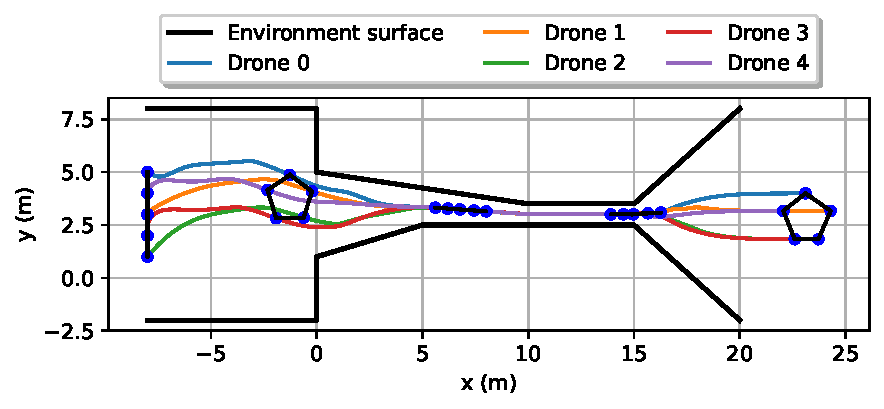
\includegraphics[width=\textwidth]{paper3/images/path_scen1.pdf}
    \caption{Scenario 1 - Motion paths}
    \end{subfigure}
    \begin{subfigure}[b]{0.495\textwidth}
    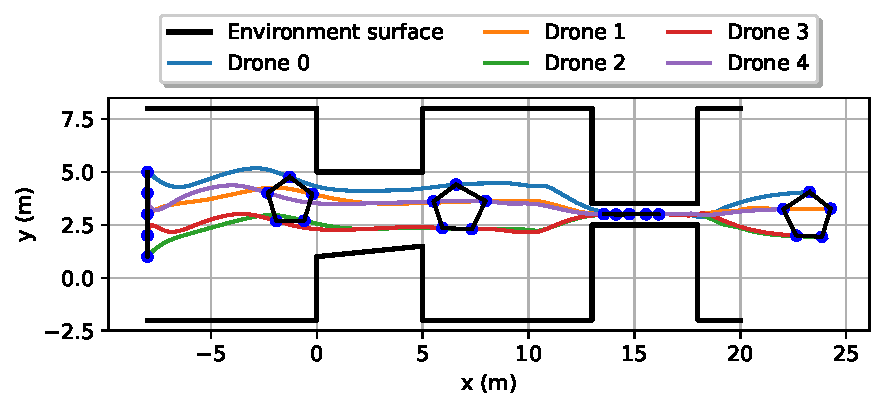
\includegraphics[width=\textwidth]{paper3/images/path_scen2.pdf}
    \caption{Scenario 2 - Motion paths}
    \end{subfigure}
    \begin{subfigure}[b]{0.495\textwidth}
    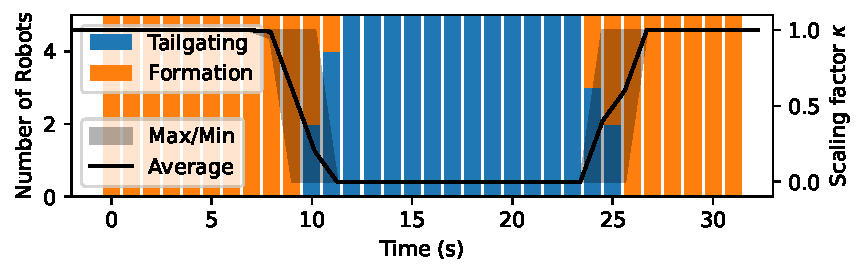
\includegraphics[width=\textwidth]{paper3/images/correlation_scen1.pdf}
    \caption{Scenario 1 - Correlation between the number of  robots (bar chart) in each mode and the scale factor (black line) over time}
    \label{fig:cor1}
    \end{subfigure}
    \begin{subfigure}[b]{0.495\textwidth}
    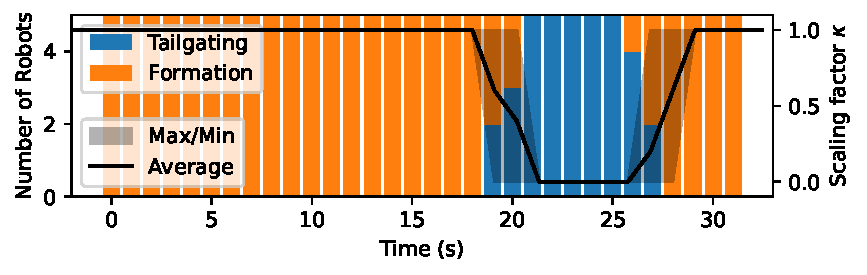
\includegraphics[width=\textwidth]{paper3/images/correlation_scen2.pdf}
    \caption{Scenario 2 - Correlation between the number of  robots (bar chart) in each mode and the scale factor (black line) over time}
    \label{fig:cor2}
    \end{subfigure}
    \caption{Trajectories and formation shapes of the robots controlled by the PRC in two evaluating scenarios.}
    \label{fig:path}
\end{figure*}

A number of simulations, comparisons, and software-in-the-loop tests have been conducted to evaluate the performance of the PRC with details as follows.

\subsection{Evaluation Setup}
The swarm includes five identical robots, each with a radius of $r=0.2$~m, a maximum speed of $\left\Vert v_\text{max}\right\Vert=1.5$~m/s, and a maximum control input $\left\Vert u_\text{max}\right\Vert=2.0$~m/s$^2$. The robot is equipped with a range sensor having the sensing range of $r_s=3$~m. The desired formation shape is set to a pentagon, the reference velocity is $\bar{v}_\text{ref}=1$~m/s, and the desired direction is $u_\text{ref}=[1,0,0]^T$. The environments include two structures, both having narrow passages, as depicted in Figure~\ref{fig:path}.

The metrics used for evaluation include the success rate, mean \textit{order} $\Phi$, mean speed (m/s), mean formation error $\varepsilon$ (m), and acceleration cost $\Gamma$ (m$^2$/s$^4$) \cite{Zhang2021}. The \textit{order} metric~\cite{Vicsek1995} measures the heading consensus of the robots and is computed as:
\begin{equation}
    \Phi=\dfrac{1}{N}\left\Vert\sum_{i=1}^N{\dfrac{v_i}{\left\Vert v_i\right\Vert}}\right\Vert
\end{equation}
Its value ranges from 0 to 1, with 1 indicating the robots have the same direction. The \textit{formation error} measures the deviation between the desired and actual positions of the robots and is calculated as~\cite{6798711}:
\begin{equation}
    \varepsilon_i = \left\Vert p_i-p^*_i\right\Vert
\end{equation} 
The acceleration cost indicates the control effort and is given by:
\begin{equation}
    \Gamma = \dfrac{1}{N}\sum_{i=1}^N{\left\Vert u_i(k)\right\Vert^2}
\end{equation} 

The comparing methods include the behavior-based reconfiguration control (BRC) \cite{Vsrhelyi2018} and the predictive formation control (PFC)~\cite{9562281}. In evaluation, each method is run 10 times for each scenario.   

\subsection{Results}
\label{subsec:results}

\begin{figure*}
    \centering
    \begin{subfigure}[b]{0.495\textwidth}
    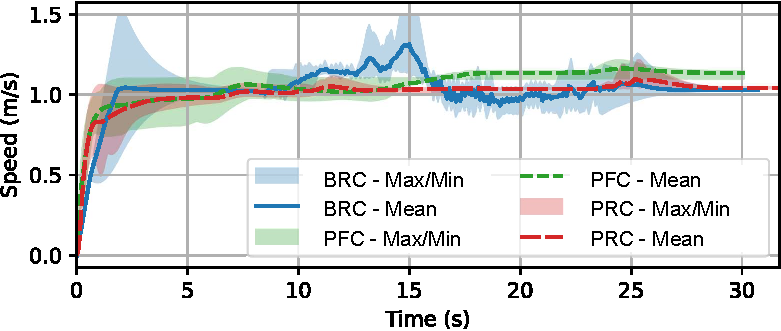
\includegraphics[width=\textwidth]{paper3/images/velocity_scen1.pdf}
    \caption{Scenario 1 - Speed}
    \label{fig:speed1}
    \end{subfigure}
    \begin{subfigure}[b]{0.495\textwidth}
    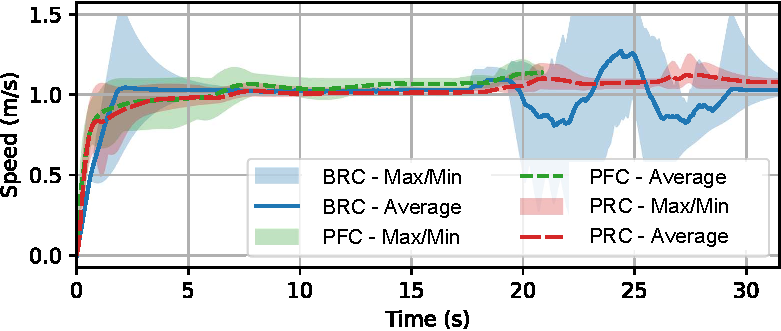
\includegraphics[width=\textwidth]{paper3/images/velocity_scen2.pdf}
    \caption{Scenario 2 - Speed}
    \label{fig:speed2}
    \end{subfigure}
    \begin{subfigure}[b]{0.495\textwidth}
    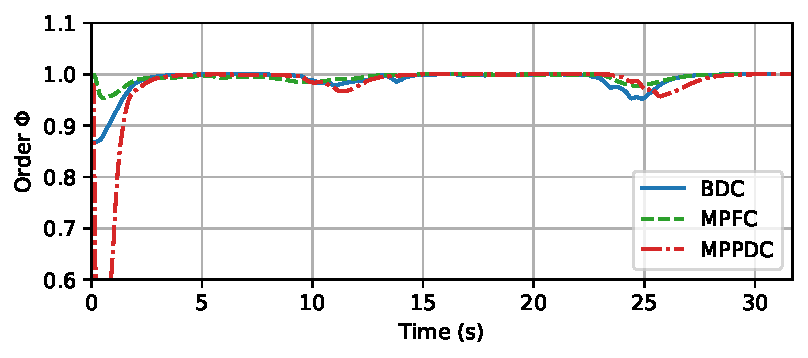
\includegraphics[width=\textwidth]{paper3/images/order_scen1.pdf}
    \caption{Scenario 1 - \textit{Order} $\Phi$}
    \label{fig:order1}
    \end{subfigure}
    \begin{subfigure}[b]{0.495\textwidth}
    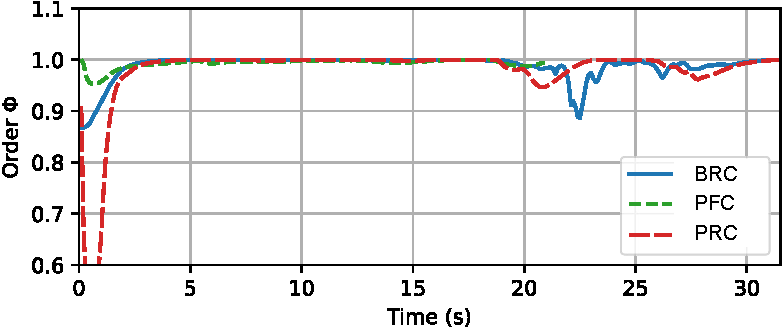
\includegraphics[width=\textwidth]{paper3/images/order_scen2.pdf}
    \caption{Scenario 2 - \textit{Order} $\Phi$}
    \label{fig:order2}
    \end{subfigure}
    \begin{subfigure}[b]{0.495\textwidth}
    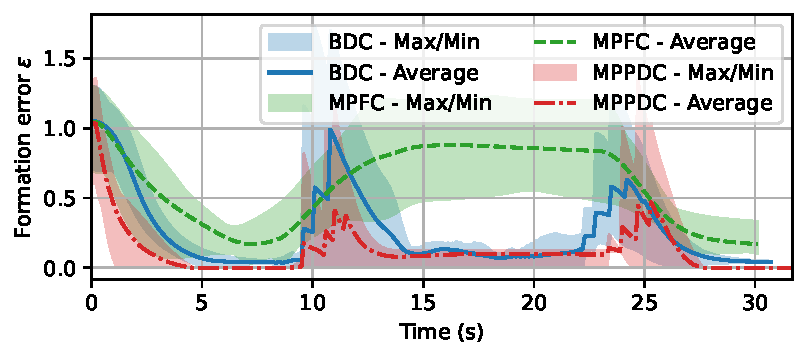
\includegraphics[width=\textwidth]{paper3/images/error_scen1.pdf}
    \caption{Scenario 1 - \textit{Formation error} $\varepsilon$}
    \label{fig:error1}
    \end{subfigure}
    \begin{subfigure}[b]{0.495\textwidth}
    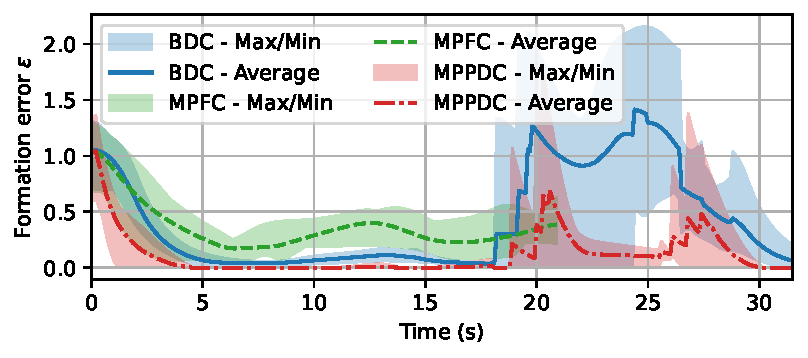
\includegraphics[width=\textwidth]{paper3/images/error_scen2.pdf}
    \caption{Scenario 2 - \textit{Formation error} $\varepsilon$}
    \label{fig:errorr2}
    \end{subfigure}
    \caption{Comparison results of three control methods in two scenarios.}
    \label{fig:comparison}
\end{figure*}

\begin{figure}
    \centering
    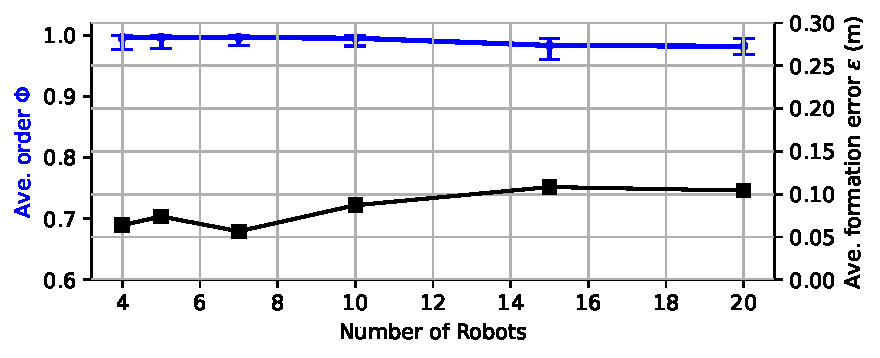
\includegraphics[width=0.8\textwidth]{paper3/images/scalability.pdf}
    \caption{Effect of the swarm size on system performance, including the mean \textit{order} $\Phi$ and formation error $\varepsilon$.}
    \label{fig:scalability}
\end{figure}

Figure \ref{fig:path} shows the formation results for both scenarios. After takeoff, the robots rapidly form the desired pentagon shape, then change their formation to pass through tight passages and finally transform back to the original desired shape. Figures~\ref{fig:cor1}-\ref{fig:cor2} depict the scaling factor $\kappa$ and the number of robots within each control mode during operation. When the environment's width is large, the scaling factor $\kappa$ stays at 1 to maintain the desired shape. As the environment narrows, $\kappa$ gradually decreases leading to more robots switching to \textit{``tailgating''} mode. The formation thus shrinks until $\kappa$ reaches 0, the point at which all robots are in \textit{``tailgating''} mode. Upon exiting the narrow corridor, $\kappa$ increases, allowing the formation to expand back to its original shape. The PRC hence provides reconfiguration capabilities for the robot swarm to adapt to complex environmental conditions.

\begin{table*}
\centering
\caption{Comparison between BRC, PFC, and the proposed PRC}
\label{tbl:analys}
\begin{tabular}{C{0.8cm}C{1.2cm}C{1.8cm}C{1.8cm}C{2.8cm}C{2.2cm}C{2.5cm}}
\hline \hline
Scen.             & Method & Success rate  & Mean \textit{order} $\Phi$ & Mean speed (m/s) ($v_\text{ref}=1$~m/s) & Mean formation error $\varepsilon$ (m) & Acceleration cost $\Gamma$ (m$^2$/s$^4$) \\ \hline
\multirow{3}{*}{1  } & BRC      & \textbf{10/10} & 0.9890     & 1.0249     & 0.3048               & 69.6589    \\
                     & PFC     & 8/10  & \textbf{0.9934}     & 1.0639     & 0.6376               & \textbf{23.7442}    \\
                     & PRC    & \textbf{10/10} & 0.9824     & \textbf{0.9863}     & \textbf{0.2423}               & 25.0894    \\ \hline
\multirow{3}{*}{2}   & BRC      & 6/10  & 0.9883     & \textbf{0.9887}     & 0.6872               & 53.8718    \\
                     & PFC     & 0/10  & \textbf{0.9953}     & 1.0470      & 0.4593               & \textbf{19.0365}    \\
                     & PRC    & \textbf{9/10}  & 0.9830     & 0.9800       & \textbf{0.3217}               & 21.8559   \\ \hline \hline
\end{tabular}
\end{table*}
 
Figure~\ref{fig:comparison} presents comparison results between the PRC and other control methods. In terms of speed, the proposed controller achieves more stable velocities with values closer to the reference $v_\text{ref}$ in both scenarios, as indicated via the average and maximum/minimum values shown in Figures~\ref{fig:speed1}-\ref{fig:speed2}. 
For the \textit{order} metric, the PRC exhibits large fluctuation at start but quickly converges to a high consensus among the robots with the \textit{order} value reaching 1, as shown in Figures~\ref{fig:order1}-\ref{fig:order2}. Both the BRC and PFC also perform well, although the BRC shows more variation than the PRC during the transition phase. In terms of formation maintenance, the PRC outperforms other methods with the smallest average error, as shown in Figures~\ref{fig:error1}-\ref{fig:errorr2}. These results are further confirmed in Table~\ref{tbl:analys}, which presents comparison data. The proposed PRC shows high performance in all metrics, with the highest success rate and the smallest formation error in both scenarios. The PFC fails in scenario 2 due to its limitation in reconfiguring the formation. The BRC has good performance in speed and mean order. It however introduces high acceleration costs, indicating that the method is not energy efficient.       

In another experiment, we vary the swarm size between 4, 5, 7, 10, 15, and 20 robots and measure the mean \textit{order} $\Phi$ and formation error $\varepsilon$ to evaluate the scalability of the proposed method. The result in Figure \ref{fig:scalability} shows that as the number of robots increases, the PRC maintains strong consensus among robots with a mean \textit{order} close to~1. The formation error, excluding the formation generation and the transition stage, remains low with variations around 0.05~m. The PRC is therefore scalable with stable performance across different swarm sizes.

\subsection{Software-in-the-loop verification}
\begin{figure*}
    \centering
    \begin{subfigure}[b]{0.56\textwidth}
    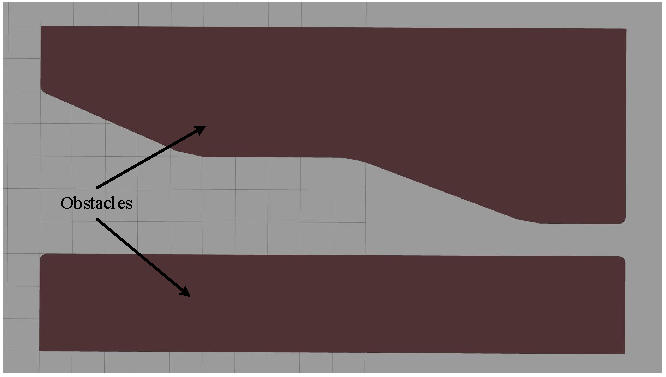
\includegraphics[width=\textwidth]{paper3/images/tunnel.pdf}
    \caption{The cave-like environment}
    \label{fig:gazebo_tunnel}
    \end{subfigure}
    \begin{subfigure}[b]{0.42\textwidth}
    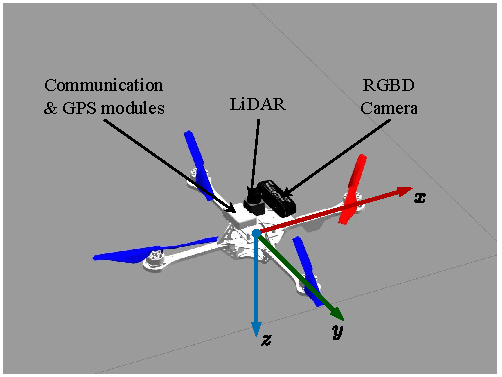
\includegraphics[width=\textwidth]{paper3/images/hummingbird.pdf}
    \caption{The drone model~\cite{Bui2022,Furrer2016}}
    \label{fig:gazebo_hummingbird}
    \end{subfigure}
    \caption{The robot and environment structure used for software-in-the-loop tests.}
    \label{fig:sil}
\end{figure*}
\begin{figure*}
    \centering
    \begin{subfigure}[b]{0.325\textwidth}
    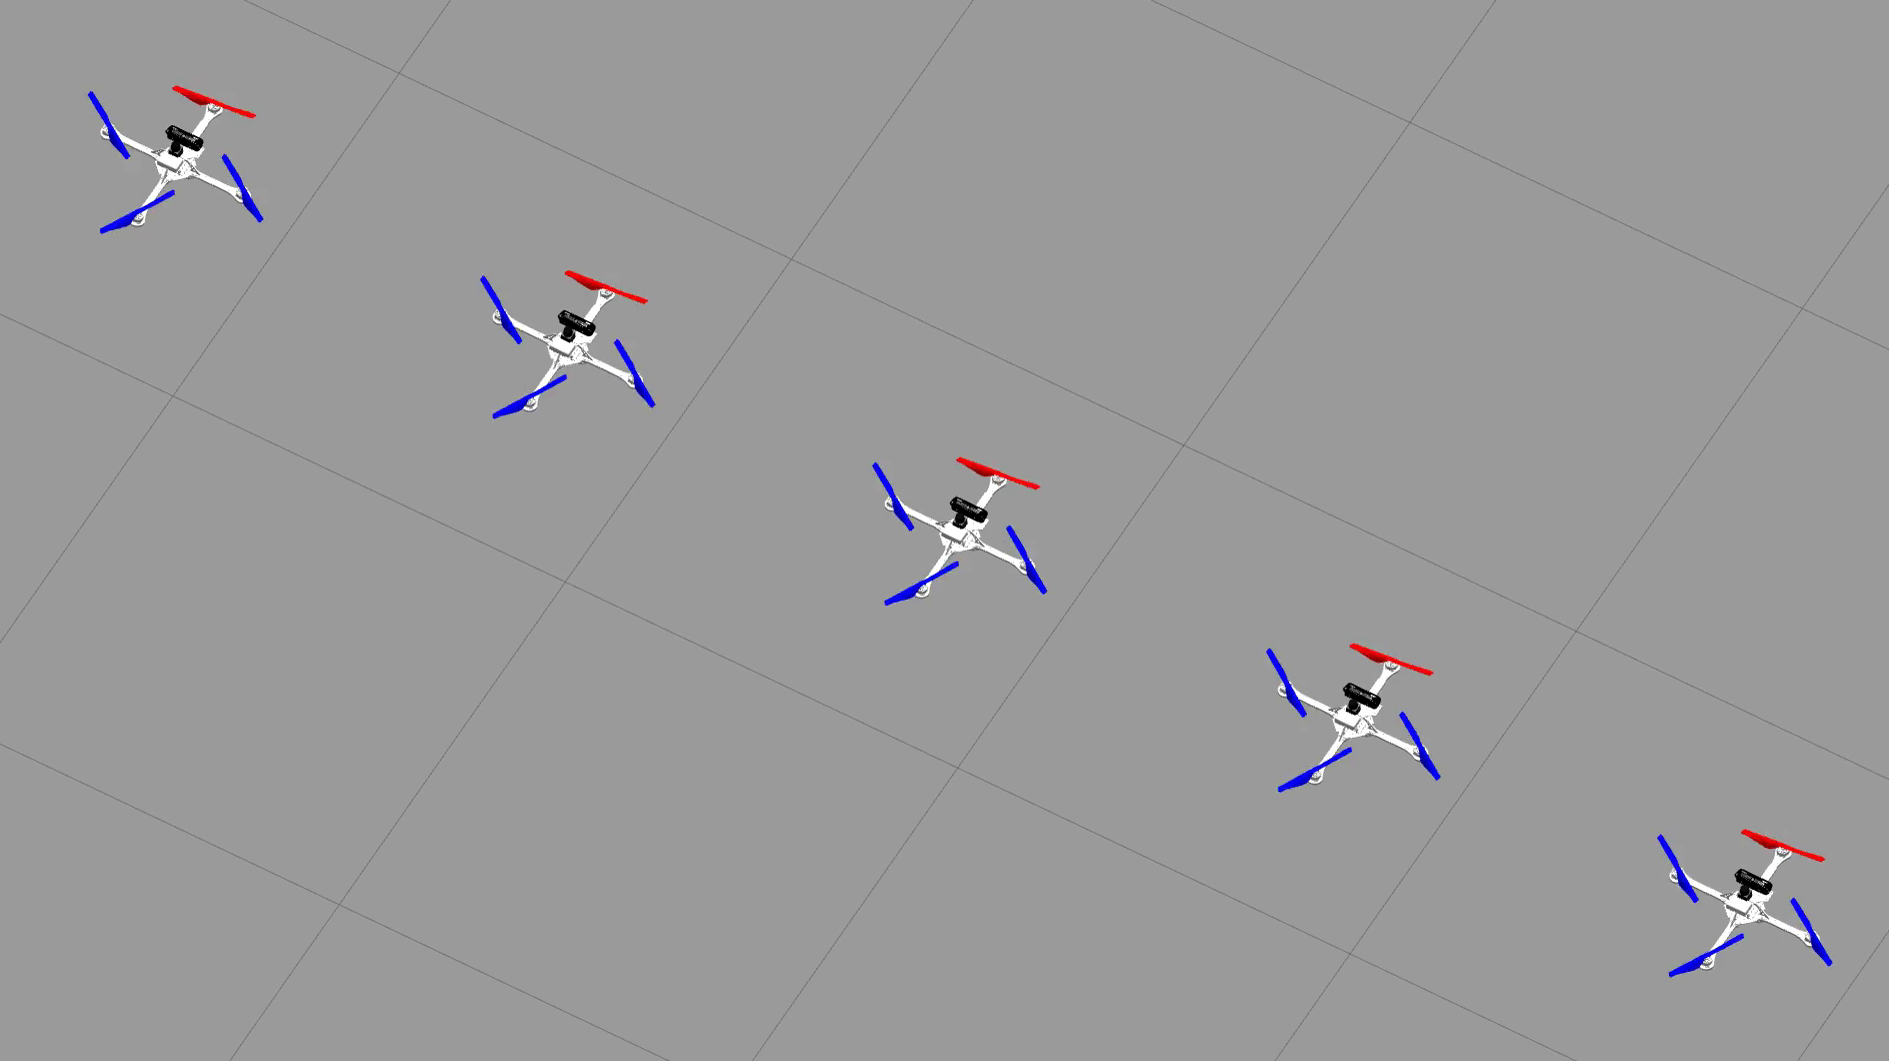
\includegraphics[width=\textwidth]{paper3/images/gazebo_01.png}
    \caption{}
    \end{subfigure}
    \begin{subfigure}[b]{0.325\textwidth}
    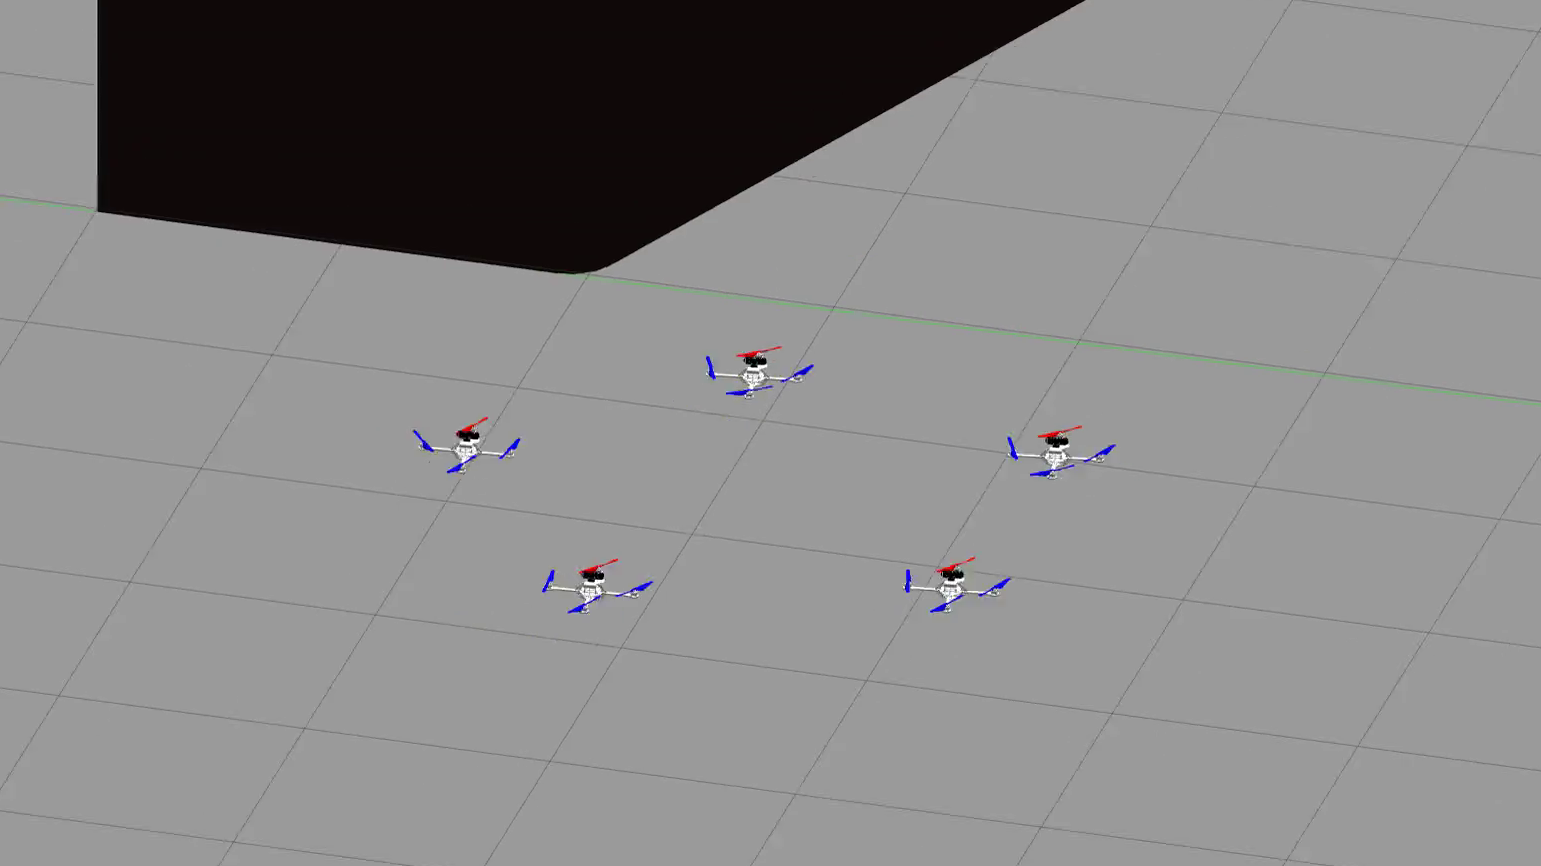
\includegraphics[width=\textwidth]{paper3/images/gazebo_02.png}
    \caption{}
    \end{subfigure}
    \begin{subfigure}[b]{0.325\textwidth}
    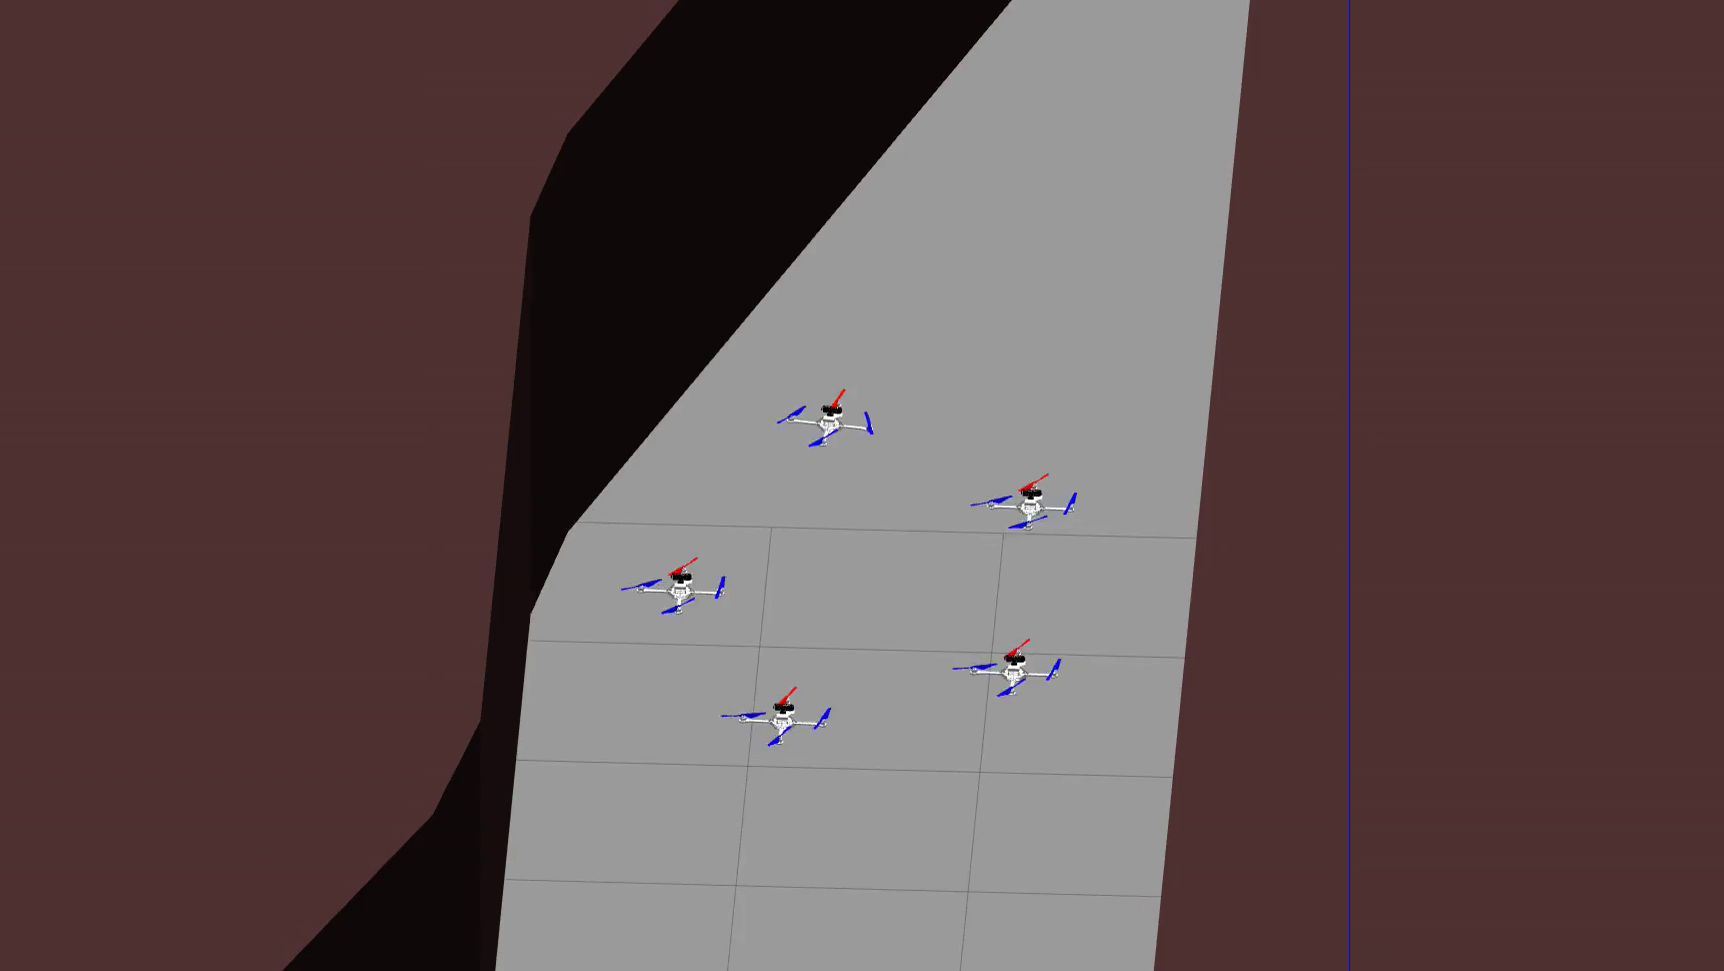
\includegraphics[width=\textwidth]{paper3/images/gazebo_03.png}
    \caption{}
    \end{subfigure}
    \begin{subfigure}[b]{0.325\textwidth}
    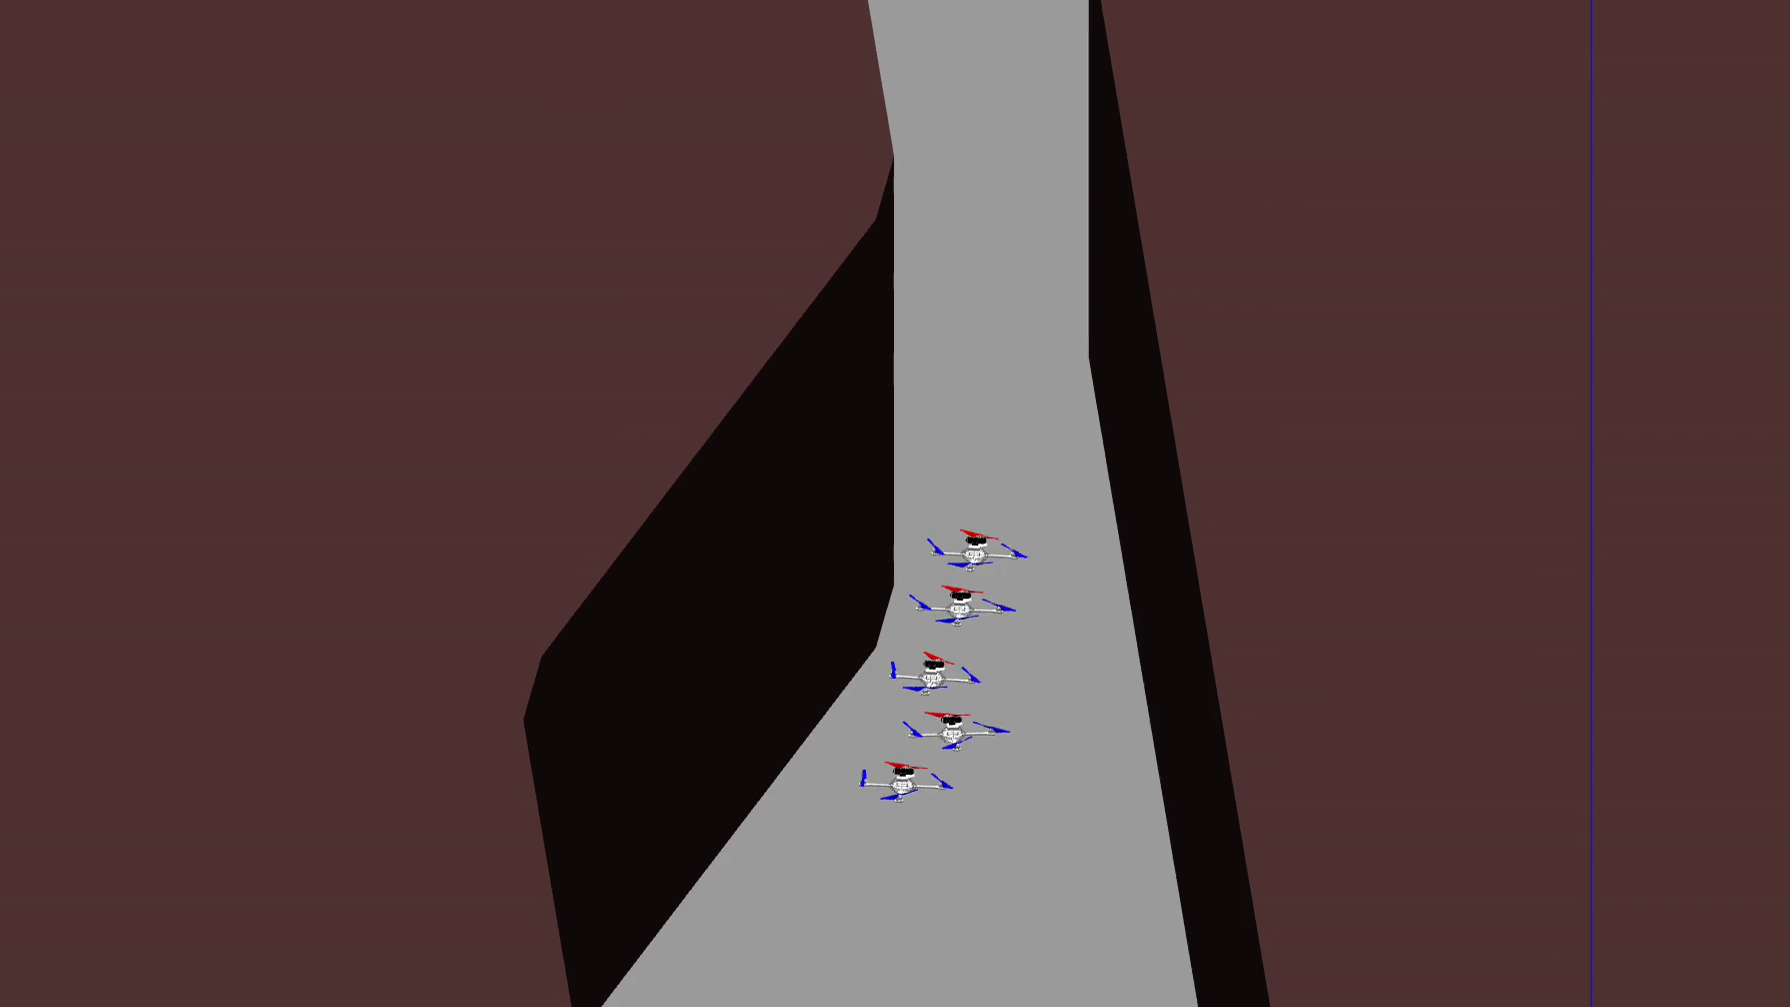
\includegraphics[width=\textwidth]{paper3/images/gazebo_04.png}
    \caption{}
    \end{subfigure}
    \begin{subfigure}[b]{0.325\textwidth}
    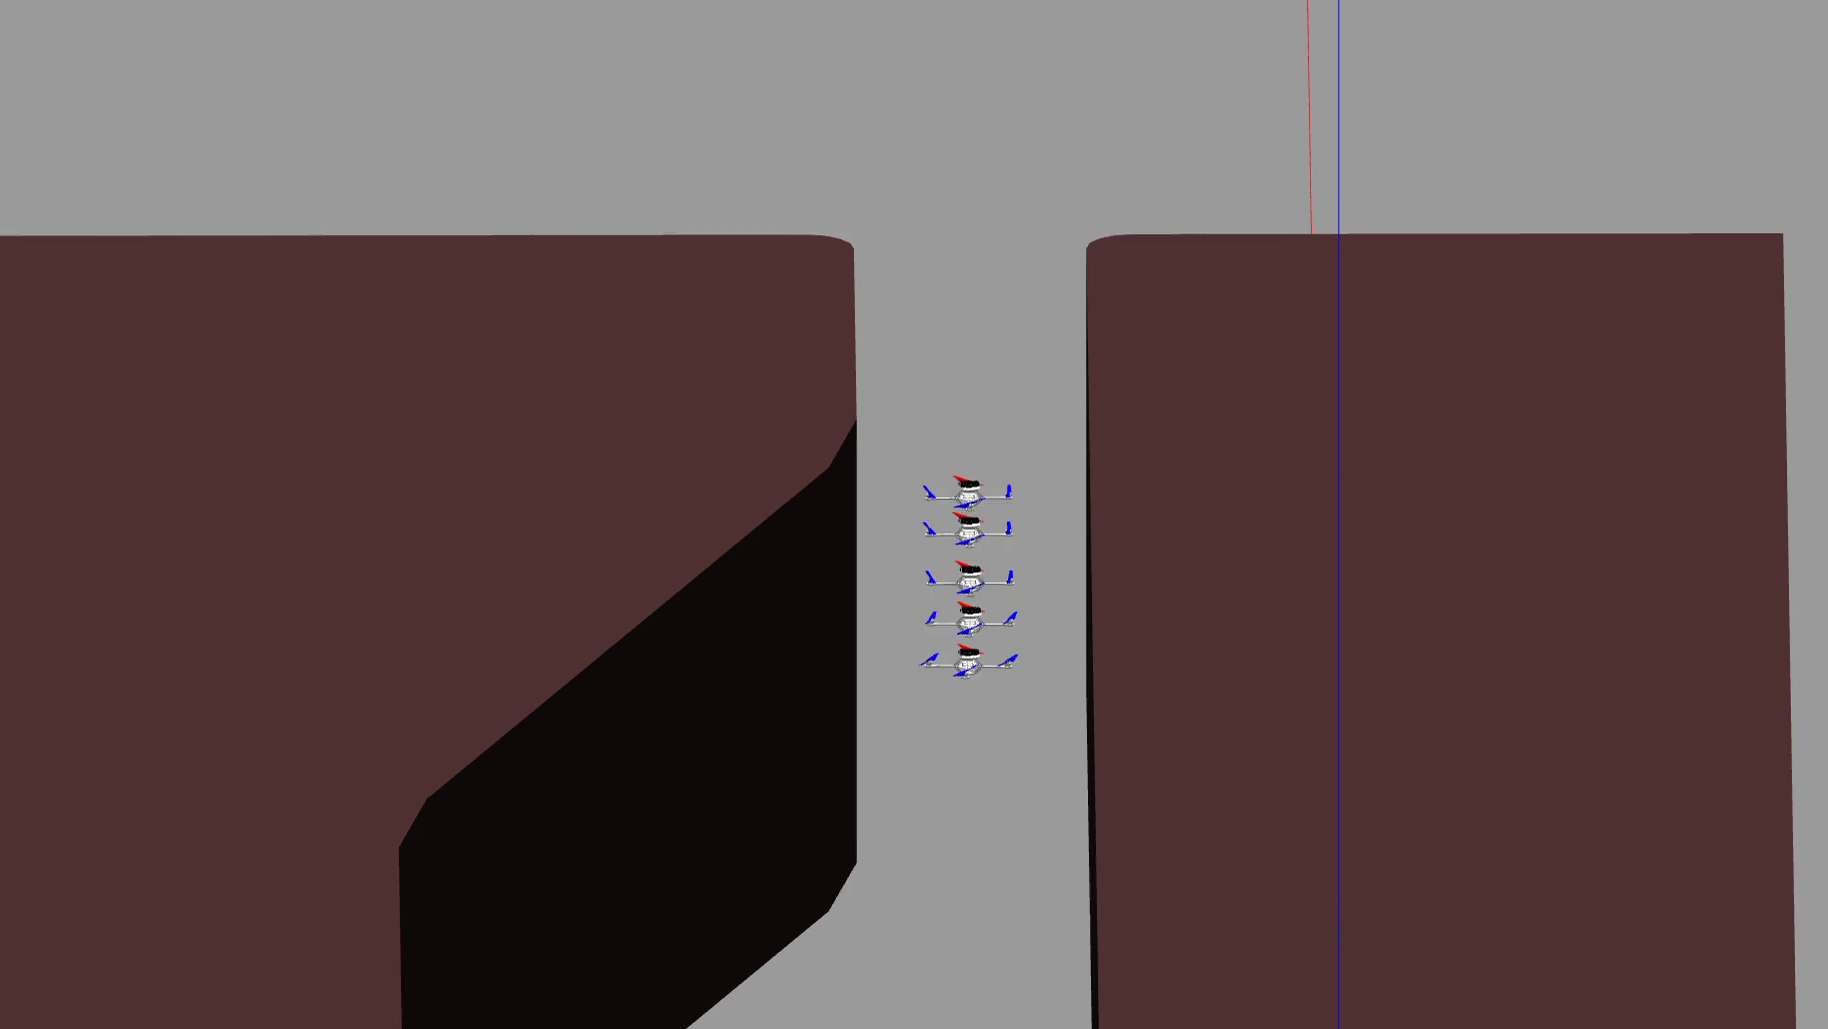
\includegraphics[width=\textwidth]{paper3/images/gazebo_05.png}
    \caption{}
    \end{subfigure}
    \begin{subfigure}[b]{0.325\textwidth}
    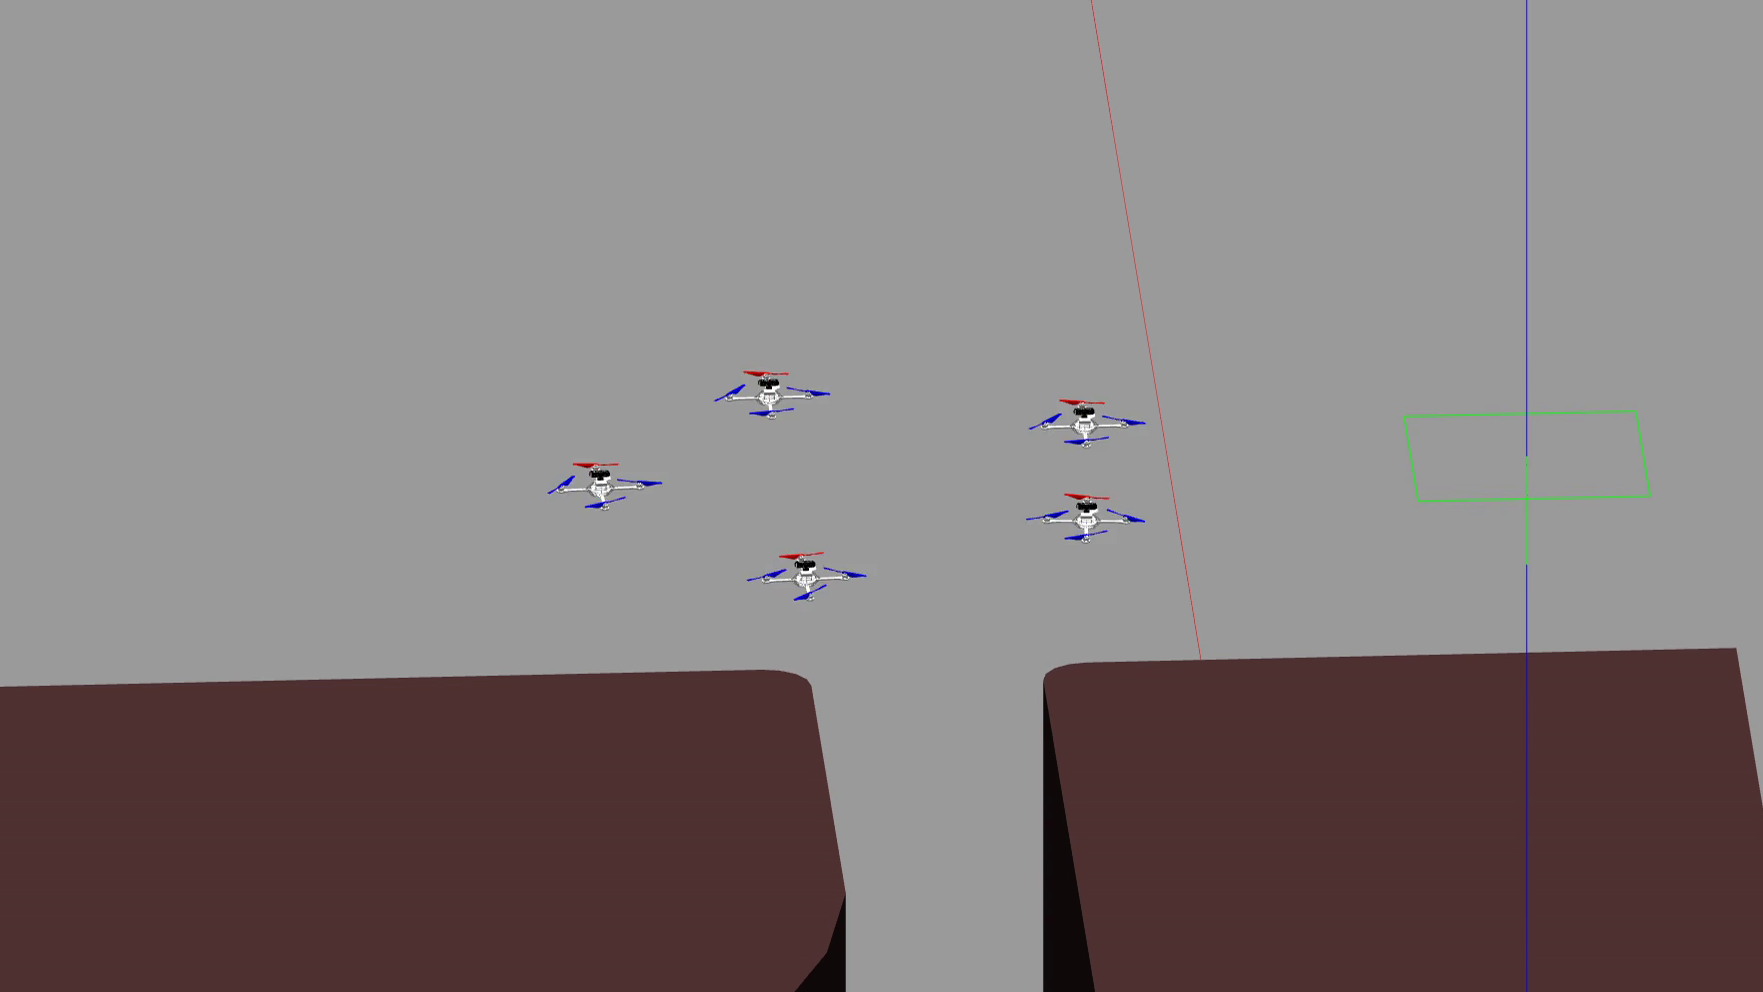
\includegraphics[width=\textwidth]{paper3/images/gazebo_06.png}
    \caption{}
    \end{subfigure}
    \caption{Reconfiguration process of the robot swarm in a SIL test: (a) initial positions of the robots; (b) form the desired pentagon shape; (c) shrink the formation in adaption to the environment; (d)-(e) switch to \textit{``tailgating''} mode to travel through the narrow passage; (f) transform back to the desired shape.}
    \label{fig:snap}
\end{figure*}

\begin{figure*}
    \centering
    \begin{subfigure}[b]{0.48\textwidth}
    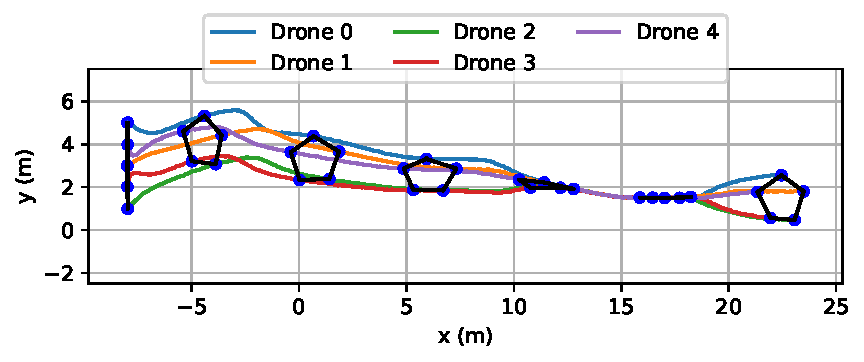
\includegraphics[width=\textwidth]{paper3/images/gazebo_path.pdf}
    \caption{The formation and motion paths}
    \label{fig:gazebo_path}
    \end{subfigure}
    \begin{subfigure}[b]{0.48\textwidth}
    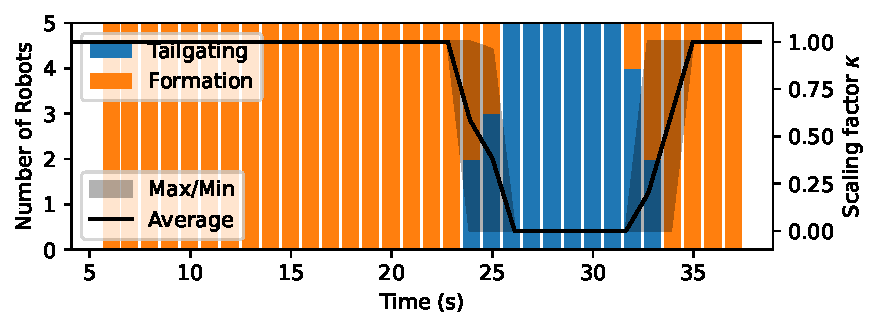
\includegraphics[width=\textwidth]{paper3/images/gazebo_correlation.pdf}
    \caption{Number of robots and scaling factor $\kappa$}
    \label{fig:gazebo_mode}
    \end{subfigure}
    \begin{subfigure}[b]{0.48\textwidth}
    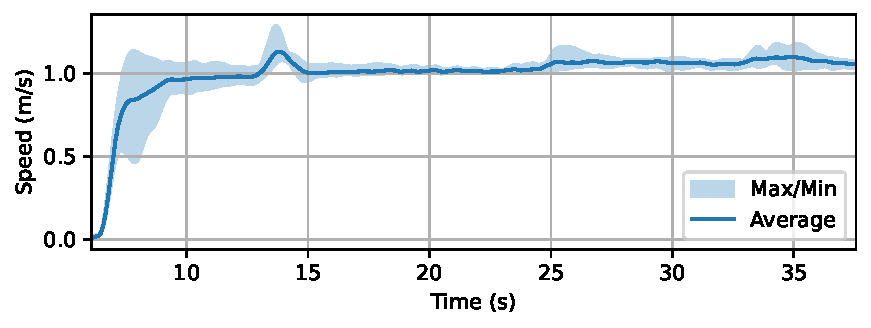
\includegraphics[width=\textwidth]{paper3/images/gazebo_speed.pdf}
    \caption{The speed profile}
    \label{fig:gazebo_speed}
    \end{subfigure}
    \begin{subfigure}[b]{0.48\textwidth}
    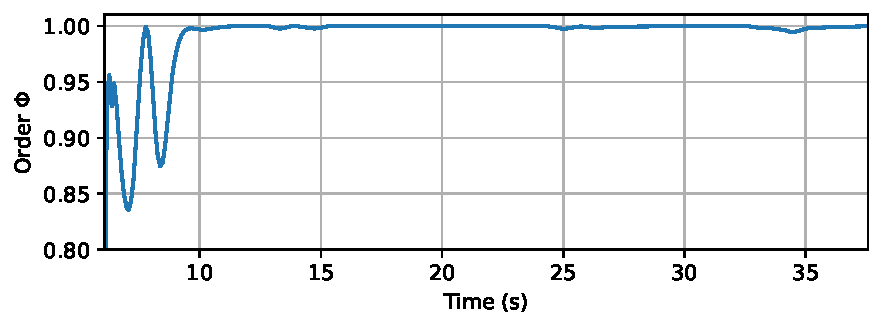
\includegraphics[width=\textwidth]{paper3/images/gazebo_order.pdf}
    \caption{The \textit{order} metric $\Phi$}
    \label{fig:gazebo_order}
    \end{subfigure}
    \begin{subfigure}[b]{0.48\textwidth}
    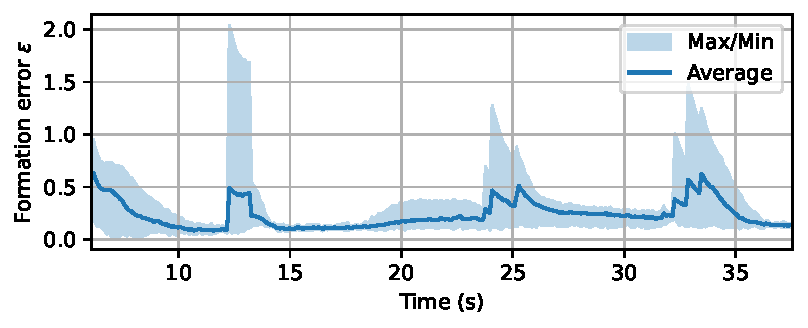
\includegraphics[width=\textwidth]{paper3/images/gazebo_error.pdf}
    \caption{The \textit{formation error} $\varepsilon_i$}
    \label{fig:gazebo_error}
    \end{subfigure}
    \begin{subfigure}[b]{0.48\textwidth}
    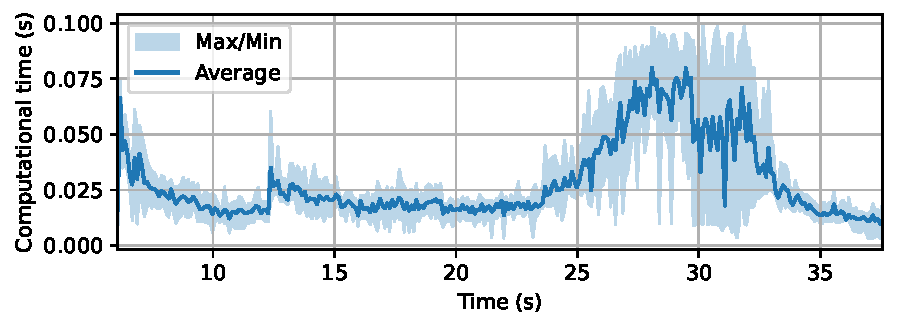
\includegraphics[width=\textwidth]{paper3/images/gazebo_computation.pdf}
    \caption{The computational time}
    \label{fig:gazebo_time}
    \end{subfigure}
    \caption{Results of the SIL tests}
    \label{fig:gazebo}
\end{figure*}

We have carried out software-in-the-loop (SIL) tests to evaluate the performance of the proposed controller in practical conditions. The environment is a narrow space that consists of two large obstacles forming a cave-like structure as shown in Figure~\ref{fig:gazebo_tunnel}. The robots include five homogeneous Hummingbird quadrotors\footnote{Source code used to setup SIL tests in Gazebo - {\tt\url{https://github.com/duynamrcv/hummingbird_simulator}}} obtained from the RotorS simulator~\cite{Furrer2016} with an arm length of 0.17~m, a mass of 0.716~kg, the rotor thrust constant of $1.6\time10^{-2}$~N/A, and the rotor drag constant of $8.54858\times10^{-6}$~Nm/A, as depicted in Figure~\ref{fig:gazebo_hummingbird}. Each robot is equipped with a range sensor to collect point cloud data of the environment, a positioning module for localization, and a communication module to interact with other robots.

Figure~\ref{fig:snap} presents the formation reconfiguration process as the swarm navigates through the environment. The robots continuously collect data about the environment and based on it adjust their formation to ensure safe operation. Figure~\ref{fig:gazebo} provides a detailed view of the result. Each UAV determines its mode and desired position based on the perception of the surrounding environment and information about its neighbors. The robots together form the relevant shape in a decentralized manner, as shown in Figures~\ref{fig:gazebo_path} - \ref{fig:gazebo_mode}. Requirements for speed, order, and formation accuracy are also met, as depicted in Figures~\ref{fig:gazebo_speed} - \ref{fig:gazebo_error}. Moreover, the computational time per controller iteration, shown in Figure~\ref{fig:gazebo_time}, indicates that the system can operate at a sampling rate of 10 Hz in the worst-case scenario, which is sufficient for real-time robot operation.

\subsection{Discussion}
Evaluation and comparison results show the key properties of the proposed control method as follows:

\subsubsection{Decentralization} The PRC is fully decentralized as each robot makes decisions based solely on its own sensor data and information from its neighbors. Unlike the approach in~\cite{AlonsoMora2018}, which requires system-wide communication to obtain information on all robots, the PRC utilizes only one-hop communication between the robot and its neighbors to update predictive states.

\subsubsection{Reliability}

The PRC can navigate the robots through complex environments with desirable performance metrics such as low formation error, stable formation direction, and high speed. Unlike previous studies ~\cite{Elkilany2020,Vsrhelyi2018,Soria2021,AlonsoMora2018} which only shrink or expand the formation to adapt to environment variations, the PRC enables the robots to completely transform to a new formation to safely maneuver through tight spaces.

\subsubsection{Scalability}
The PRC can operate with different swarm sizes, for example from 4 to 20 robots, without requiring any modifications to the algorithm. It maintains reliable performance and consistent metric values across various swarm sizes. 

\subsubsection{Robustness}
The PRC provides robustness to operate in different environmental structures. Through real-time data obtained from local sensors and communication networks, the swarm can dynamically expand, shrink, or transform into a line shape to optimize its ability to navigate through narrow spaces.
\section{Conclusion}\label{sec:conclusion}
In this work, we have presented an optimal predictive reconfiguration control method to guide a swarm of robots through cluttered environments with varying path widths. The controller features two modes, \textit{``formation''} and \textit{``tailgating''}, and a scaling factor that enable the swarm to adapt its shape to environmental conditions. A set of cost functions is introduced to enforce formation constraints and safety requirements while enabling state prediction for enhanced control performance. Evaluation results show that the proposed controller effectively navigates the robot swarm through complex environments with narrow passages. The control performance is superior in most evaluation metrics compared to two other state-of-the-art methods. Software-in-the-loop tests further confirm the validity and practicability of the proposed controller.

